\documentclass[../improvements.tex]{subfiles}

\begin{document}

  論理合成の結果から, クリティカルパスが EX ステージにあることが分かった.
  そのクリティカルパスは以下の通りである.
  \begin{displaymath}
    \begin{aligned}
      &1. ID/EX パイプラインレジスタ \\
      \rightarrow &2. ALU のオペランドと制御信号の生成 \\
      \rightarrow &3. ALU における演算 \\
      \rightarrow &4. 分岐予測の答え合わせと分岐の判断 \\
      \rightarrow &5. ID ステージのフラッシュ \\
      \rightarrow &6. ID/EX パイプラインレジスタ
    \end{aligned}
  \end{displaymath}

  上記のクリティカルパスを短縮するために, 以下のことを行った.
  \begin{enumerate}
    \item ALU のオペランドの生成を ID ステージで行う (\ref{subsubsection:ex-to-id} 章)
    \item パイプラインフラッシュをパイプラインレジスタで行う (\ref{subsubsection:rethink-flush} 章)
  \end{enumerate}

  \subsubsection{ALU のオペランドの生成を ID ステージで行う} \label{subsubsection:ex-to-id}
  EX ステージで演算を行う前に, 以下のオペランドと制御信号を用意する必要がある.
  \begin{enumerate}
    \item オペランド
      \begin{enumerate}
        \item ALU の演算のオペランド \label{item:alu-in}
        \item 比較専用 ALU の演算のオペランド \label{item:branch-alu-in}
      \end{enumerate}
    \item 制御信号
      \begin{enumerate}
        \item ALU に対して演算の種類を指定する制御信号 \label{item:alu-op}
        \item 比較専用 ALU に対して比較の種類を指定する制御信号 \label{item:branch-alu-op}
      \end{enumerate}
  \end{enumerate}
  倫理合成の結果から, 信号が生成されるまでに必要な時間から, 
  演算のオペランド (\ref{item:alu-in} と \ref{item:branch-alu-in}) の生成がボトルネックになっていた.
  これを改善するために, 演算のオペランドの生成回路を ID ステージに移動させた.

  その結果, クリティカルパスの 2 である「ALU のオペランドと制御信号の生成」が「ALU の制御信号の生成」になり, 
  プロセッサの最小動作クロック周期を $9ns$ から $8ns$ まで減らすことができた.
  それでも, プログラムの実行時間が, まだ分岐予測を導入する前より長いため, 次の改善を実施した.

  \subsubsection{パイプラインフラッシュをパイプラインレジスタで行う} \label{subsubsection:rethink-flush}
  実装していたパイプラインフラッシュの回路では, 
  プログラムの実行の中で分岐が起きた時に, 
  パイプラインレジスタではなく, IF ステージと ID ステージのフラッシュをステージ内で行っていた (図 \ref{fig:critical-path-before}).
  これにより, ID ステージの命令がデータメモリと汎用レジスタに対する書き込み信号の生成タイミングは
  分岐結果が出た後のタイミングになってしまう.
  分岐結果が分かるまでに ID ステージは待たないといけないため, 無駄な時間が生じてしまう.

  \begin{figure*}
    \centering
    \begin{subfigure}{\columnwidth}
      \centering
      \resizebox{0.9\columnwidth}{!}{
        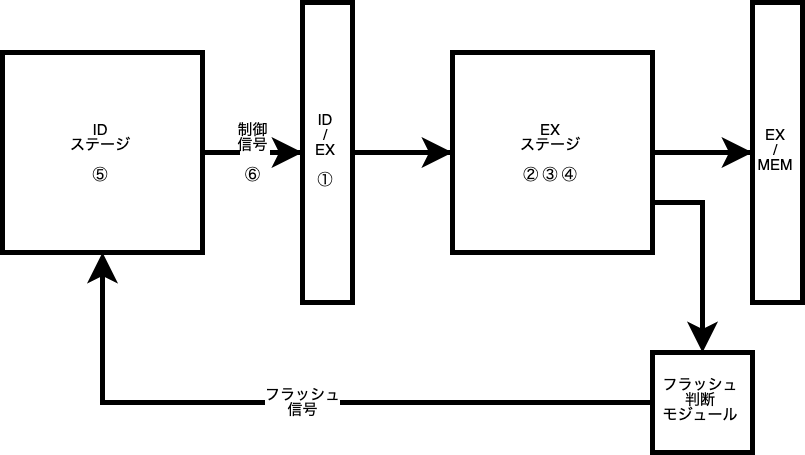
\includegraphics{../../images/critical_path_before.png}
      }
      \caption{改善前}
      \label{fig:critical-path-before}
    \end{subfigure}
    \begin{subfigure}{\columnwidth}
      \centering
      \resizebox{0.9\columnwidth}{!}{
        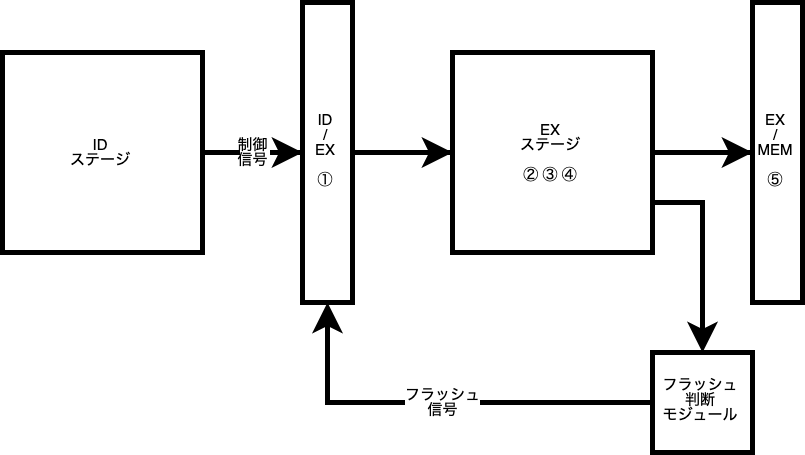
\includegraphics{../../images/critical_path_after.png}
      }
      \caption{改善後}
      \label{fig:critical-path-after}
    \end{subfigure}
    \caption{パイプラインフラッシュ処理の回路とクリティカルパス}
  \end{figure*}

  これを改善するために, パイプラインのフラッシュをステージ内ではなく, 
  パイプラインレジスタで行うようにした (図 \ref{fig:critical-path-after}).
  改善後の回路では, たとえば ID ステージで「データメモリに対して書き込む」信号が生成されても, 
  EX ステージの分岐結果が「分岐する」なら, 
  その信号が ID/EX パイプラインレジスタに保存される前に, 「データメモリに対して書き込まない」へと無効化される.

  この改善によってクリティカルパスが以下のように短くなった. 
  \begin{displaymath}
    \begin{aligned}
      &1. ID/EX パイプラインレジスタ \\
      \rightarrow &2. ALU のオペランドと制御信号の生成 \\
      \rightarrow &3. ALU における演算 \\
      \rightarrow &4. 分岐予測の答え合わせと分岐の判断 \\
      \rightarrow &5. EX/MEM パイプラインレジスタ
    \end{aligned}
  \end{displaymath}
  そして, プロセッサの最小動作クロック周期を $8ns$ から $5ns$ まで減らすことができた.
  改善によって得られたクロック周期は分岐予測導入前の $6ns$ よりも短くなったので, 
  分岐予測機能を今回のプロセッサの設計に導入してもいいと判断した.

  \subsubsection{クリティカルパスの短縮後の論理合成}
  クリティカルパスの短縮を行った後の性能評価の結果を表 \ref{table:logic-synthesis-improved} にまとめた.
  クリティカルパスの短縮により, 分岐予測の実装によって $9ns$ までに増えたクロック周期を
  $5ns$ へと減少させることができた.

  \begin{table*}[t]
    \centering
    \begin{tabular}{|c|r|r|r|}
    \hline
    プロセッサ & \multicolumn{1}{c|}{最小動作クロック周期 {[}$ns${]}} & \multicolumn{1}{c|}{面積 {[}$\mu m^2${]}} & \multicolumn{1}{c|}{消費電力 {[}$mW${]}} \\ \hline
    分岐予測実装前 & 6 & 357534.7228 & 7.5732 \\
    分岐予測実装後 & 9 & 936675.8334 & 10.6318 \\
    クリティカルパス短縮後 & 5 & 764805.1213 & 15.3567 \\ \hline
    \end{tabular}
    \caption{性能改善前後の論理合成の結果}
    \label{table:logic-synthesis-improved}
  \end{table*}

  \subsubsection{更に改善できる点}
  後二週間があれば, 1つのステージ内の処理を細分化して複数個のステージで行うように, 
  パイプラインのステージを増やすことをやってみたかった.
  1つのステージ内の処理負担が減少すれば, クリティカルパスも短くなるだろう.
  それによってプロセッサのクロック周期を更に短くできるのではないかと考えている.

\end{document}
